\section{Software State Machines}

\important{SEP Handouts: 08\_FSM\_Example}

\subsection{Introduction - FSM in Hardware vs Software}

\begin{definition}{Finite State Machine (FSM)}
A machine with a finite number of states and transitions, which responds to inputs based on its current state. It represents a computational model used to design both computer programs and sequential logic circuits. FSMs are particularly useful in embedded systems for controlling the behavior of the system in response to external events.
\end{definition}

\begin{theorem}{Hardware FSM}
    \begin{itemize}
        \item Flip-Flops store internal state
        \item Clock-driven: Inputs evaluated at clock edges, state changes only on clock edges
    \end{itemize}
    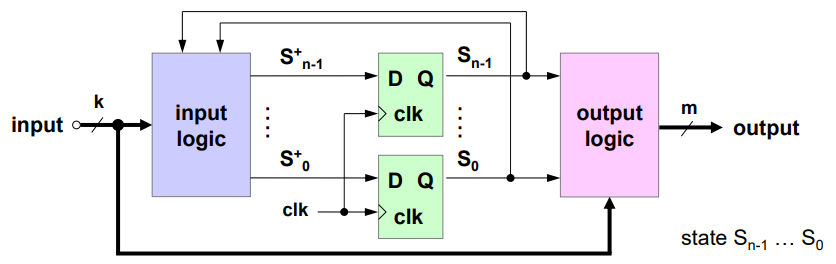
\includegraphics[width=\linewidth]{hardwarefsm.png}
    \begin{itemize}
    \item Intrinsically parallel - multiple FSMs process simultaneously
    \item Unchanged input signals create no overhead
    \item Typically implemented as either Moore or Mealy machines
\end{itemize}
\end{theorem}

\begin{corollary}{Moore vs Mealy FSMs}
    \begin{itemize}
        \item Moore FSM: Outputs depend only on current state
        \item Mealy FSM: Outputs depend on current state and inputs
    \end{itemize}
    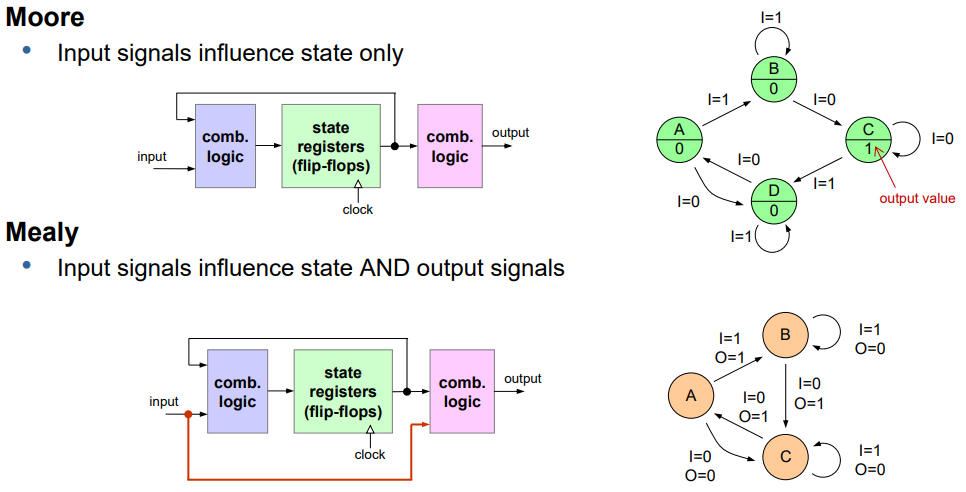
\includegraphics[width=\linewidth]{mealy_vs_moore.png}
\end{corollary}

\begin{concept}{Software FSM is different!}\\
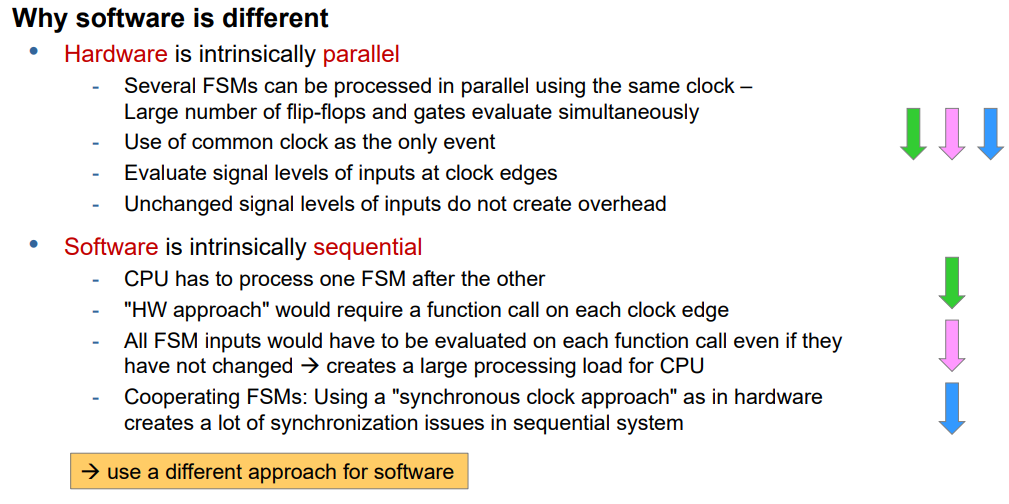
\includegraphics[width=0.9\linewidth]{hardqwarevssoftwarefsm.png}
\end{concept}

\subsection{Reactive Systems}

\begin{definition}{Reactive System (State-Event Model)}
A system that responds to external events (inputs) based on its internal state. It is event-driven and processes events as they occur, rather than evaluating all inputs periodically. Reactive systems are particularly well-suited for implementing FSMs in software because they minimize CPU overhead.
\end{definition}

\begin{concept}{Components of a Reactive System}
\begin{itemize}
    \item \textbf{Events:} External inputs that trigger the system's response
    \item \textbf{Internal state:} Memory of what happened before
    \item \textbf{Actions:} Influence on the outside world (outputs)
    \item \textbf{Transitions:} Rules for how events change state and trigger actions
\end{itemize}

The key advantage of the reactive approach is that the FSM is evaluated only when an input changes, reducing processing overhead compared to polling all inputs regularly.
\end{concept}

\begin{example2}
{Common applications of state-event models}
\begin{itemize}
    \item Communication protocols (connection establishment, data transfer, connection termination)
    \item Human-machine interfaces (input recognition and validation)
    \item Parsing of programming languages and text
    \item Process control systems (washing machines, vending machines, heating systems)
    \item Embedded control systems (automotive, medical devices)
\end{itemize}
\end{example2}

\raggedcolumns
\columnbreak

\subsection{Modeling State Machines in UML}

\begin{definition}{UML State Diagram}
A graphical representation based on the Unified Modeling Language (UML) for modeling finite state machines. Based on the notation developed by Prof. David Harel, it describes the reactive behavior of systems. UML state diagrams provide a standard way to document and communicate the behavior of state-based systems.
\end{definition}

\begin{concept}{UML State Diagram Elements}
\begin{itemize}
    \item \textbf{State:} Internal condition of the system waiting for the next event
    \item \textbf{Event:} Asynchronous input that may cause a transition
    \item \textbf{Transition:} Reaction to an event, may change state and/or trigger an action
    \item \textbf{Action:} Output associated with a transition (written after a forward slash)
    \item \textbf{Initial state:} Default starting state of the system (indicated by a solid circle)
    \item \textbf{Default transition:} Arrow from initial state to the first active state
\end{itemize}
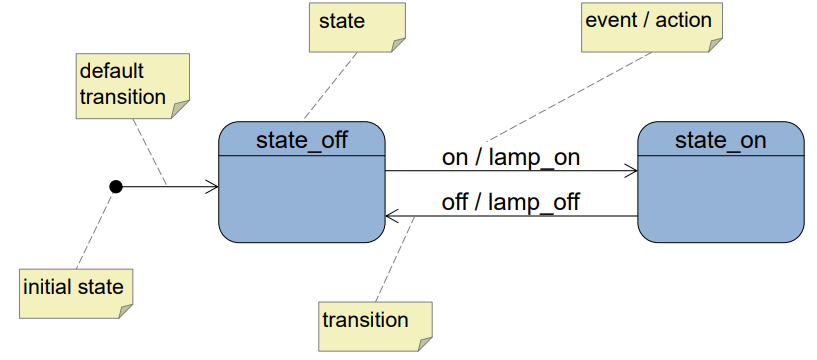
\includegraphics[width=0.5\linewidth]{umlfsmexample.png}

In contrast to hardware FSM notations like Mealy, UML state diagrams:
\begin{itemize}
    \item Treat inputs as asynchronous events rather than signal levels
    \item Treat outputs as actions
    \item Omit inputs that have no effect (increasing diagram clarity)
    \item Can represent both Mealy and Moore behaviors in a unified notation
\end{itemize}
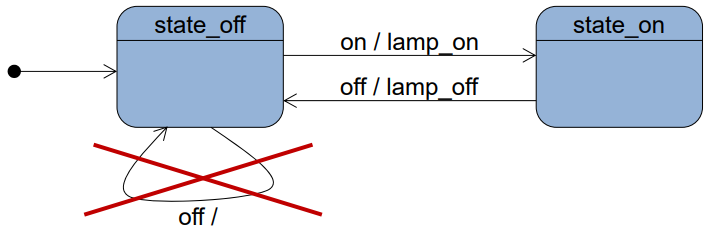
\includegraphics[width=0.4\linewidth]{incontrasttomealynotation.png}
\end{concept}

\begin{KR}{UML State Diagram erstellen}
    \paragraph{Grundelemente}
    \begin{itemize}
        \item States (Zustände): Rechtecke mit Namen
        \item Transitions (Übergänge): Pfeile zwischen States
        \item Initial State: Gefüllter Kreis mit Pfeil
        \item Events: Auslöser für Transitions
        \item Actions: Aktionen bei Transitions
    \end{itemize}
    
    \paragraph{Transition-Syntax}
    Event / Action
    \begin{itemize}
        \item Event: Was löst den Übergang aus
        \item Action: Was wird beim Übergang ausgeführt
        \item Beispiel: \texttt{start / water\_on, timer\_start}
    \end{itemize}
    
    \paragraph{Vorgehen}
    \begin{enumerate}
        \item Alle Zustände identifizieren
        \item Events (Eingaben) definieren
        \item Actions (Ausgaben) definieren
        \item Übergänge zwischen Zuständen zeichnen
        \item Initial State festlegen
        \item Entry/Exit Actions definieren (falls nötig)
    \end{enumerate}
    
    \paragraph{Regeln beachten}
    \begin{itemize}
        \item Jeder State muss erreichbar sein
        \item Determinismus: Eindeutige Transitions
        \item Vollständigkeit: Alle Events behandeln
    \end{itemize}
\end{KR}



\begin{example}
Simple light switch state diagram in UML:

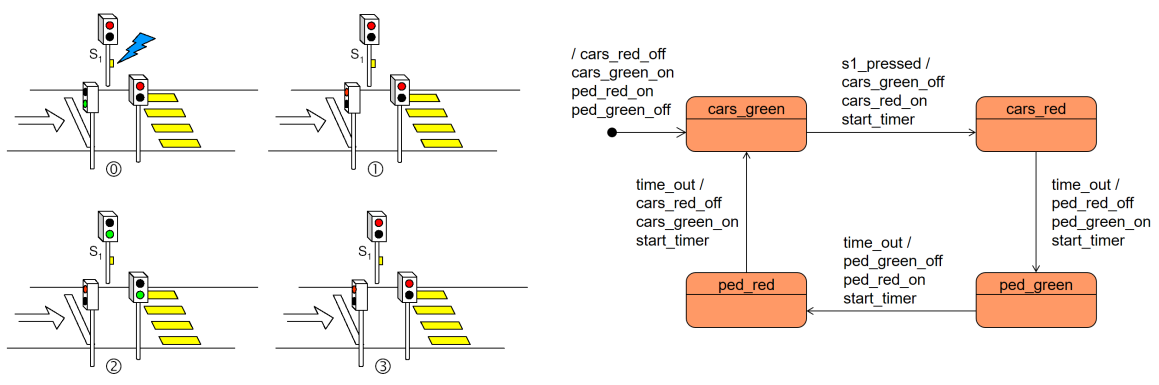
\includegraphics[width=\linewidth]{lightsignalfsmexampel.png}

With an initial default transition to state\_off.

Note that the transition "off" in state\_off is not shown because it would have no effect and trigger no action.
\end{example}

\begin{example2}{Autowaschanlage State Machine}
    Spezifikation:
    \begin{itemize}
        \item Ruhezustand wartet auf Start
        \item Drei Schritte: wash, rinse, dry (je gleich lang)
        \item wash: Wasser + Shampoo
        \item rinse: nur Wasser  
        \item dry: nur Luftstrom
        \item Stop-Taste bricht ab $\rightarrow$ alles aus, zurück zu Rest
    \end{itemize}
    
    \tcblower
    
    \textbf{Events:}
    \begin{itemize}
        \item start: Starttaste gedrückt
        \item stop: Stoptaste gedrückt
        \item time\_out: Timer abgelaufen
    \end{itemize}
    
    \textbf{Actions:}
    \begin{itemize}
        \item water\_on/off, shampoo\_on/off, air\_on/off
        \item timer\_start
    \end{itemize}
    
    \textbf{State Diagram:}\\
    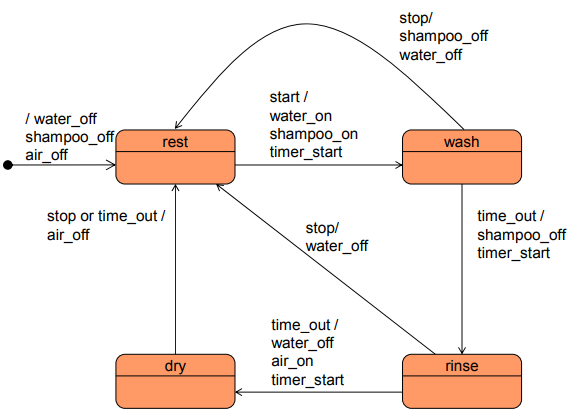
\includegraphics[width=0.6\linewidth]{waschanlage_state_diagram.png}
    \begin{itemize}
        \item \textbf{rest}: Ausgangszustand
        \item \textbf{wash}: start / water\_on, shampoo\_on, timer\_start
        \item \textbf{rinse}: time\_out / shampoo\_off, timer\_start
        \item \textbf{dry}: time\_out / water\_off, air\_on, timer\_start
        \item Zurück zu rest: stop / water\_off, shampoo\_off, air\_off
    \end{itemize}
\end{example2}



\subsection{Interaction of FSMs}

\begin{definition}{FSM Interaction Components}
\begin{itemize}
    \item \textbf{Port:} Defines the messages that can be sent and received by an FSM
        \begin{itemize}
            \item Output message $\rightarrow$ action of the FSM
            \item Input message $\rightarrow$ event for the FSM
        \end{itemize}
    \item \textbf{Link:} Defines a connection for sending messages between FSMs
    \item \textbf{Event Queue:} Buffer for events generated by different objects
\end{itemize}
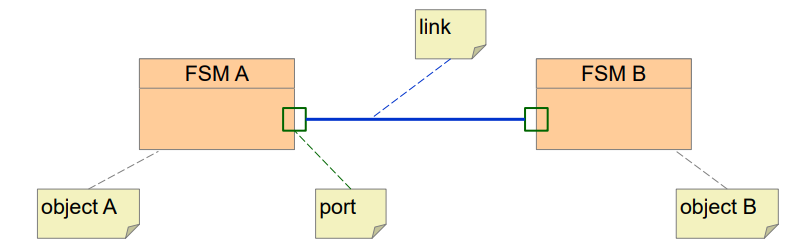
\includegraphics[width=0.6\linewidth]{portlinkfsm.png}
\end{definition}

\begin{example2}{Reactive System Partitioned into two FSMs}\\
    Interaction of FSMs happens through event messages.\\
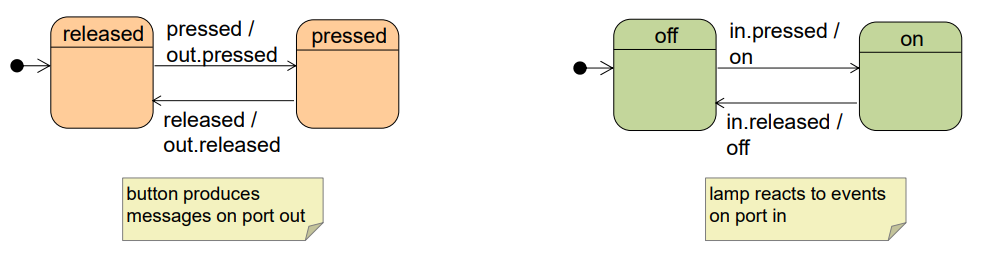
\includegraphics[width=0.8\linewidth]{fsmexamplepartitioned.png}
\end{example2}

\begin{concept}{Event Queue for FSM Interaction}
\begin{itemize}
    \item Collects events generated by different objects
    \item Buffered to avoid losing events (especially important in interrupt-driven systems)
    \item FSM processes one event after the other
    \item Events are deleted after processing
    \item Provides decoupling between event producers and consumers
\end{itemize}
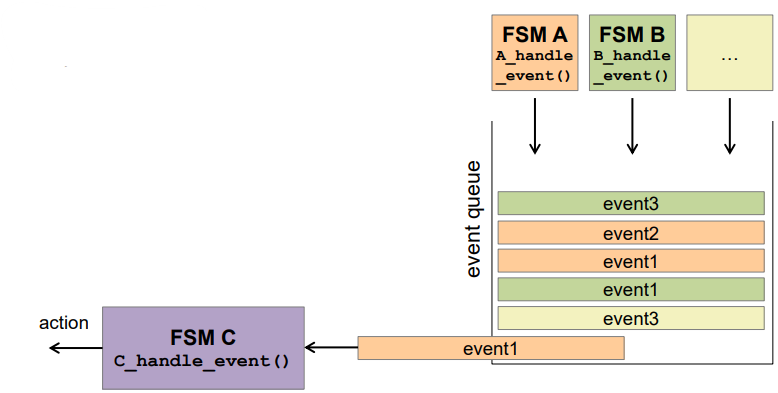
\includegraphics[width=0.8\linewidth]{eventqueuefms.png}

Actions of one FSM become events for another FSM, allowing complex systems to be constructed from simpler components. This approach enables modular design and clear separation of concerns.
\end{concept}



\begin{KR}{Building Event-Based FSM Systems}
\paragraph{System Structure}
\begin{itemize}
    \item Divide system into multiple FSMs with well-defined responsibilities
    \item Define ports and interfaces for each FSM
    \item Connect FSMs through links and event queues
    \item Keep individual FSMs simple and focused on specific tasks
\end{itemize}

\paragraph{Implementation}
\begin{itemize}
    \item Use interrupt service routines (ISRs) to capture hardware events
    \item ISRs place events in queue rather than processing directly
    \item Main program continuously checks queue and dispatches events to appropriate FSMs
    \item Each FSM processes events according to its current state
    \item Ensure thread safety if multiple cores or interrupts are involved
\end{itemize}

\paragraph{Benefits}
\begin{itemize}
    \item Clear separation of concerns
    \item Improved maintainability
    \item Reduced complex interdependencies
    \item More predictable system behavior
    \item Easier to test individual components
    \item Supports incremental development
\end{itemize}
\end{KR}

\subsection{Conclusion and Best Practices}

\begin{concept}{Key Differences: Software vs Hardware FSMs}
\begin{itemize}
    \item Software FSMs are event-driven rather than clock-driven
    \item Software FSMs process one event at a time, while hardware FSMs can be parallel
    \item Software FSMs often use a state-event model for efficiency
    \item Software FSMs can use more complex data structures and conditions
    \item Interaction between software FSMs typically uses message passing
\end{itemize}
\end{concept}

\begin{KR}{FSM Design Best Practices}
\paragraph{Design Phase}
\begin{itemize}
    \item Start with a clear, well-defined problem statement
    \item Identify all possible states the system can be in
    \item Define all events that can occur and how they affect each state
    \item Use UML state diagrams to visualize and document the FSM
    \item Review for completeness, consistency, and determinism
\end{itemize}

\paragraph{Implementation Phase}
\begin{itemize}
    \item Keep state handling code separate from event detection
    \item Use enumerations for states and events to improve readability
    \item Keep ISRs short and move complex processing to the main loop
    \item Use event queues for communication between FSMs
    \item Consider using a table-driven approach for complex FSMs
\end{itemize}

\paragraph{Testing and Debugging}
\begin{itemize}
    \item Test each state transition individually
    \item Verify correct behavior for unexpected or illegal events
    \item Add debug output for state transitions during development
    \item Consider adding state history for troubleshooting
    \item Test boundary conditions and error cases
\end{itemize}
\end{KR}


\begin{remark}
    State Machines eignen sich besonders für reaktive Systeme mit klaren Zuständen und definierten Übergängen. Die Trennung von Event-Detection, State-Logic und Actions macht den Code wartbar und testbar.
\end{remark} 
\raggedcolumns
\columnbreak

\subsection{Implementation in C}

\begin{concept}{Basic Implementation Structure}
Software implementation of an FSM typically uses two main functions:
\begin{itemize}
    \item \textbf{fsm\_init():} Initializes the state machine to its default state
    \item \textbf{fsm\_handle\_event(event):} Processes an incoming event based on current state
\end{itemize}
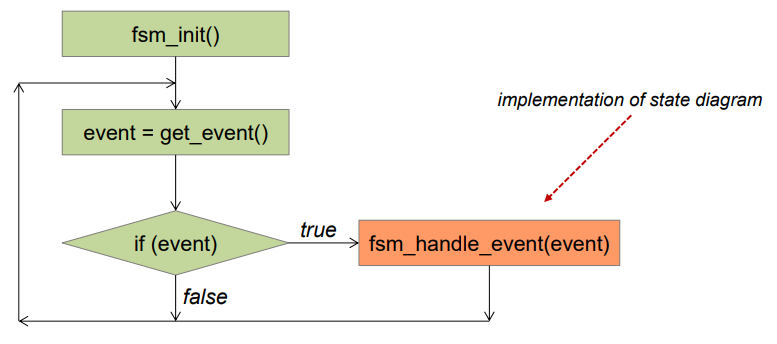
\includegraphics[width=0.8\linewidth]{cfsm.png}

The main program continuously polls for events and passes them to the state machine when they occur. This separation of event detection and processing is key to the efficiency of software FSMs.
\end{concept}

\begin{KR}{State Machine in C implementieren}

    \begin{minipage}{0.45\linewidth}
    \paragraph{Datenstrukturen}
    \begin{itemize}
        \item Enum für States: \\ \texttt{typedef enum \{STATE1, STATE2\} state\_t;}
        \item Enum für Events: \\ \texttt{typedef enum \{EVENT1, EVENT2\} event\_t;}
        \item Statische Variable: \\ \texttt{static state\_t current\_state;}
    \end{itemize}
    \vspace{5mm}
    \paragraph{Hauptschleife}
\begin{lstlisting}[language=C, style=basesmol]
int main(void) {
    event_t event;
    fsm_init();
    while (1) {
        event = get_event();
        if (event != NO_EVENT) {
            fsm_handle_event(event);
        }
    }
}
\end{lstlisting}
    \end{minipage}
    \hspace{4mm}
    \begin{minipage}{0.5\linewidth}
    \paragraph{FSM Handler (Switch-Case)}
\begin{lstlisting}[language=C, style=basesmol]
void fsm_handle_event(event_t event) {
    switch (current_state) {
        case STATE1:
            switch (event) {
                case EVENT1:
                    action1();
                    current_state = STATE2;
                    break;
                default:
                    // unbehandelte Events
                    break;
            }
            break;
        case STATE2:
            // ...
            break;
        default:
            current_state = INITIAL_STATE;
            break;
    }
}
\end{lstlisting}
\end{minipage}

\paragraph{Event Detection}
    \begin{itemize}
        \item Polling: Regelmäßige Abfrage in Hauptschleife
        \item Interrupt-driven: Events in ISR in Queue einreihen
        \item Edge Detection: Flanken erkennen (static Variable)
    \end{itemize}
\end{KR}

\begin{code}{FSM Implementation Pattern}
\begin{lstlisting}[language=C, style=basesmol]
// State and event enumerations
typedef enum {
    STATE_A,
    STATE_B,
    STATE_C,
    // ...other states
} state_t;

typedef enum {
    NO_EVENT,
    EVENT_X,
    EVENT_Y,
    // ...other events
} event_t;

// Current state variable
static state_t state;

// Initialization function
void fsm_init(void) {
    state = STATE_A;  // Set initial state
    // Additional initialization if needed
}

// Event handler function
void fsm_handle_event(event_t event) {
    switch (state) {
        case STATE_A:
            switch (event) {
                case EVENT_X:
                    action1();
                    state = STATE_B;
                    break;
                case EVENT_Y:
                    action2();
                    // No state change
                    break;
                default:
                    // Event ignored in this state
                    break;
            }
            break;
        case STATE_B:
            // Handle events for state B
            break;
        // Other states
    }
}

// Main loop
int main(void) {
    event_t event;
    
    fsm_init();
    
    while (1) {
        event = get_event();
        if (event != NO_EVENT) {
            fsm_handle_event(event);
        }
    }
}
\end{lstlisting}
\end{code}










